\documentclass{ximera}

\title{Graphing Activity}
\author{MATH 425: Calculus I}

\begin{document}
\begin{abstract}
    Working with the peers in your group, solve the following problems. Make sure to show and justify all your work. Make sure everyone in the group understands the solution and participates. Be prepared to report your answers to the whole class. 
\end{abstract}
\maketitle


\begin{exercise}
    Determine if any of the following statements are true or false.  Explain your reasoning. (If your answer is false, an example may be enough explanation.  If your answer is true, an example is not enough.)
    \begin{enumerate}
        \item Every relative maximum and minimum of a function $h$ occurs at a point $c$ where $h'(c)$ is either zero or does not exist.\\
        This statement is TRUE or FALSE (circle one) because \dots
        \item At every point $c$ where $h'(c)$ is zero or does not exist, the function $h$ has a relative maximum or minimum.\\
        This statement is TRUE or FALSE (circle one) because \dots
    \end{enumerate}
\end{exercise}

\begin{exercise}
    Suppose that $g(x)$ is a function that is continuous for every value of $x\neq 2$ whose first derivative is 
    $$g'(x)=\frac{(x+4)(x-1)(2x-2)}{x-2}.$$
    Further, note that $g$ has a vertical asymptote at $x=2$. 
    \begin{enumerate}
        \item Determine all critical numbers of $g(x)$.
        \item By developing a carefully labeled first derivative sign chart, decide whether $g(x)$ has a local maximum, local minimum, or neither at each critical number.
        \item Does $g$ have a global maximum?  Global minimum?  Justify your claims.
        \item Sketch a possible graph of $y=g(x)$. (Focus on shape rather than exact points included on the graph.)
        \begin{image}
            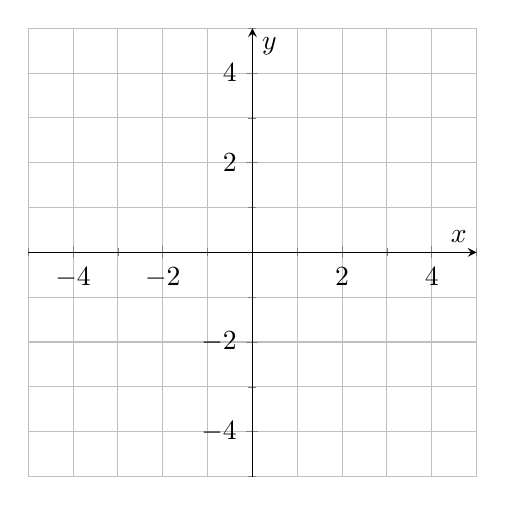
\begin{tikzpicture}
  \begin{axis}[
    axis lines=middle,
    xlabel={$x$},
    ylabel={$y$},
    xmin=-5, xmax=5,
    ymin=-5, ymax=5,
    grid=both,
    minor tick num=1,
    axis equal image,
    view={0}{90},
  ]

  \end{axis}
\end{tikzpicture}
        \end{image}
        %\xmalt{A blank coordinate plane ranging from -5 to +5 on the $x$-axis and $y$-axis.}
    \end{enumerate}
\end{exercise}

\begin{exercise}
    Suppose that $g$ is a function whose second derivative $g''$ is given by the graph below. 
    \begin{image}
        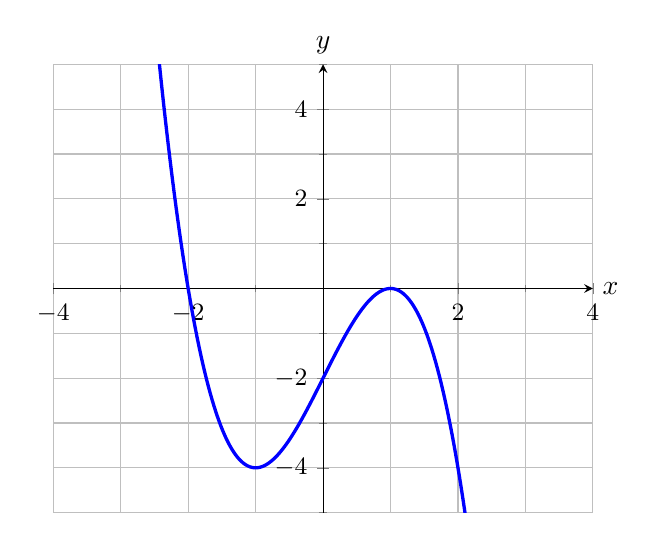
\begin{tikzpicture}
  \begin{axis}[
    axis lines = middle,
    xlabel = {$x$},
    ylabel = {$y$},
    xmin = -4, xmax = 4,
    ymin = -5, ymax = 5,
    grid = both,
    minor tick num = 1,
    ticklabel style={font=\small},
    every axis x label/.style={at={(current axis.right of origin)}, anchor=west},
    every axis y label/.style={at={(current axis.above origin)}, anchor=south},
  ]

    % Graph of y = -(x-1)^2(x+2)
    \addplot[
      domain=-4:4,
      samples=300,
      very thick,
      blue,
    ]
    { -((x - 1)^2) * (x + 2) };

  \end{axis}
\end{tikzpicture}
    \end{image}
    %\xmalt{A graph of what looks like a cubic polynomial with negative leading coefficient. Direction changes at the points $(-1,-4)$ and $(1,0)$.  Zeros of the graph are at $(-2,0)$ and $(1,0)$.  The $y$-intercept is at $(0,-2)$. }
    \begin{enumerate}
         \item Find the $x$-coordinates of all points of inflection for $g$.
    \item Fully describe the concavity of $g$ by making an appropriate sign chart.
    \item Suppose you are given the information that $g'(-2)=0$.  Is there a local maximum, local minumum, or neither for the function $g$ at this critical number, or is it impossible to say?  why?
    \item Assumeing that $g''(x)$ is a polynomial (and that all important behavior of $g''$ is seen in the graph above). what degree polynomial do you think $g(x)$ is?  Why?
    \end{enumerate}
   
\end{exercise}





\end{document}